\documentclass{standalone}
\usepackage{tikz}
\usetikzlibrary{patterns, positioning}


\begin{document}
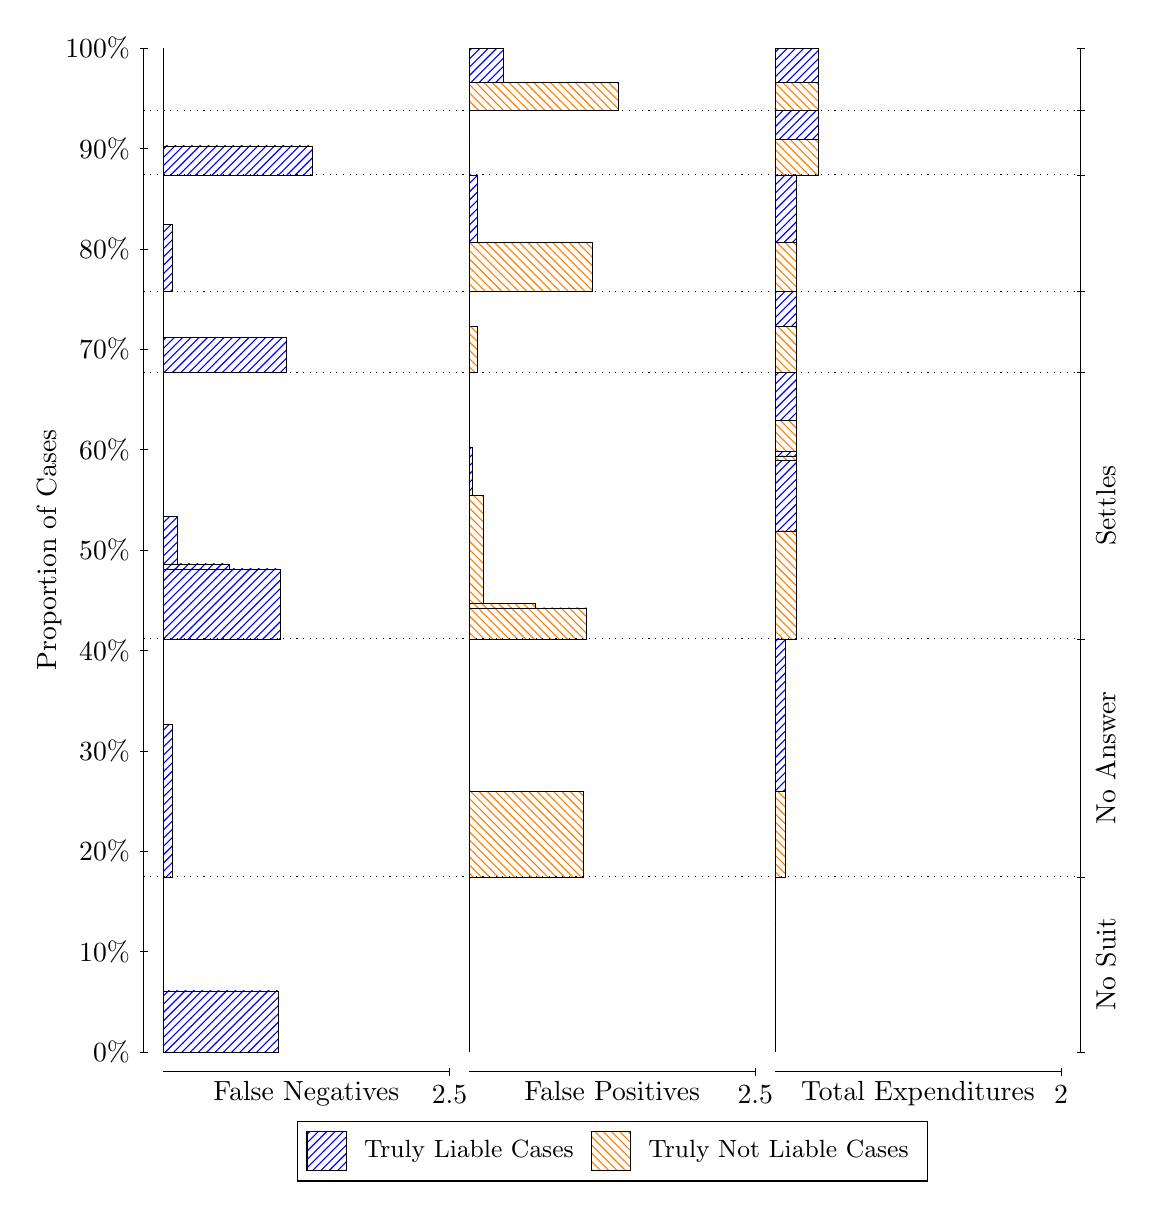
\begin{tikzpicture}
\draw[black, very thin] (1.5,1.75) -- (1.5,14.5);
\node[rotate=90, text=black, anchor=center] at (0.3, 8.125) {Proportion of Cases};
\draw[black, very thin] (1.45,1.75) -- (1.55,1.75);
\node[text=black, anchor=east] at (1.45, 1.75) {0\%};
\draw[black, very thin] (1.45,3.025) -- (1.55,3.025);
\node[text=black, anchor=east] at (1.45, 3.025) {10\%};
\draw[black, very thin] (1.45,4.3) -- (1.55,4.3);
\node[text=black, anchor=east] at (1.45, 4.3) {20\%};
\draw[black, very thin] (1.45,5.575) -- (1.55,5.575);
\node[text=black, anchor=east] at (1.45, 5.575) {30\%};
\draw[black, very thin] (1.45,6.85) -- (1.55,6.85);
\node[text=black, anchor=east] at (1.45, 6.85) {40\%};
\draw[black, very thin] (1.45,8.125) -- (1.55,8.125);
\node[text=black, anchor=east] at (1.45, 8.125) {50\%};
\draw[black, very thin] (1.45,9.4) -- (1.55,9.4);
\node[text=black, anchor=east] at (1.45, 9.4) {60\%};
\draw[black, very thin] (1.45,10.675) -- (1.55,10.675);
\node[text=black, anchor=east] at (1.45, 10.675) {70\%};
\draw[black, very thin] (1.45,11.95) -- (1.55,11.95);
\node[text=black, anchor=east] at (1.45, 11.95) {80\%};
\draw[black, very thin] (1.45,13.225) -- (1.55,13.225);
\node[text=black, anchor=east] at (1.45, 13.225) {90\%};
\draw[black, very thin] (1.45,14.5) -- (1.55,14.5);
\node[text=black, anchor=east] at (1.45, 14.5) {100\%};

\draw[black, very thin] (13.4,1.75) -- (13.4,14.5);
\draw[black, very thin] (13.35,1.75) -- (13.45,1.75);
\node[anchor=west] at (13.35, 1.75) {};
\draw[black, very thin] (13.35,3.9731) -- (13.45,3.9731);
\node[anchor=west] at (13.35, 3.9731) {};
\draw[black, very thin] (13.35,6.9967) -- (13.45,6.9967);
\node[anchor=west] at (13.35, 6.9967) {};
\draw[black, very thin] (13.35,10.379) -- (13.45,10.379);
\node[anchor=west] at (13.35, 10.379) {};
\draw[black, very thin] (13.35,11.408) -- (13.45,11.408);
\node[anchor=west] at (13.35, 11.408) {};
\draw[black, very thin] (13.35,12.89) -- (13.45,12.89);
\node[anchor=west] at (13.35, 12.89) {};
\draw[black, very thin] (13.35,13.707) -- (13.45,13.707);
\node[anchor=west] at (13.35, 13.707) {};
\draw[black, very thin] (13.35,14.5) -- (13.45,14.5);
\node[anchor=west] at (13.35, 14.5) {};

\draw[black, very thin, pattern color=blue, pattern=north east lines] (1.75,1.75) rectangle (3.2033,2.5268);
\draw[black, very thin, pattern color=orange, pattern=north west lines] (1.75,2.5268) rectangle (1.75,3.9731);
\draw[black, very thin, pattern color=blue, pattern=north east lines] (1.75,3.9731) rectangle (1.859,5.9135);
\draw[black, very thin, pattern color=orange, pattern=north west lines] (1.75,5.9135) rectangle (1.75,6.9967);
\draw[black, very thin, pattern color=blue, pattern=north east lines] (1.75,6.9967) rectangle (3.2397,7.8863);
\draw[black, very thin, pattern color=blue, pattern=north east lines] (1.75,7.8863) rectangle (2.5857,7.9475);
\draw[black, very thin, pattern color=blue, pattern=north east lines] (1.75,7.9475) rectangle (1.9317,8.553);
\draw[black, very thin, pattern color=orange, pattern=north west lines] (1.75,8.553) rectangle (1.75,10.379);
\draw[black, very thin, pattern color=blue, pattern=north east lines] (1.75,10.379) rectangle (3.3123,10.825);
\draw[black, very thin, pattern color=orange, pattern=north west lines] (1.75,10.825) rectangle (1.75,11.408);
\draw[black, very thin, pattern color=blue, pattern=north east lines] (1.75,11.408) rectangle (1.859,12.263);
\draw[black, very thin, pattern color=orange, pattern=north west lines] (1.75,12.263) rectangle (1.75,12.89);
\draw[black, very thin, pattern color=blue, pattern=north east lines] (1.75,12.89) rectangle (3.6393,13.257);
\draw[black, very thin, pattern color=orange, pattern=north west lines] (1.75,13.257) rectangle (1.75,13.707);
\draw[black, very thin, pattern color=orange, pattern=north west lines] (1.75,13.707) rectangle (1.75,14.066);
\draw[black, very thin, pattern color=blue, pattern=north east lines] (1.75,14.066) rectangle (1.75,14.5);
\draw[black, very thin, pattern color=orange, pattern=north west lines] (5.6333,1.75) rectangle (5.6333,3.1963);
\draw[black, very thin, pattern color=blue, pattern=north east lines] (5.6333,3.1963) rectangle (5.6333,3.9731);
\draw[black, very thin, pattern color=orange, pattern=north west lines] (5.6333,3.9731) rectangle (7.0867,5.0563);
\draw[black, very thin, pattern color=blue, pattern=north east lines] (5.6333,5.0563) rectangle (5.6333,6.9967);
\draw[black, very thin, pattern color=orange, pattern=north west lines] (5.6333,6.9967) rectangle (7.123,7.3892);
\draw[black, very thin, pattern color=orange, pattern=north west lines] (5.6333,7.3892) rectangle (6.469,7.451);
\draw[black, very thin, pattern color=orange, pattern=north west lines] (5.6333,7.451) rectangle (5.815,8.823);
\draw[black, very thin, pattern color=blue, pattern=north east lines] (5.6333,8.823) rectangle (5.6697,9.4285);
\draw[black, very thin, pattern color=blue, pattern=north east lines] (5.6333,9.4285) rectangle (5.6333,10.379);
\draw[black, very thin, pattern color=orange, pattern=north west lines] (5.6333,10.379) rectangle (5.7423,10.962);
\draw[black, very thin, pattern color=blue, pattern=north east lines] (5.6333,10.962) rectangle (5.6333,11.408);
\draw[black, very thin, pattern color=orange, pattern=north west lines] (5.6333,11.408) rectangle (7.1957,12.035);
\draw[black, very thin, pattern color=blue, pattern=north east lines] (5.6333,12.035) rectangle (5.7423,12.89);
\draw[black, very thin, pattern color=orange, pattern=north west lines] (5.6333,12.89) rectangle (5.6333,13.341);
\draw[black, very thin, pattern color=blue, pattern=north east lines] (5.6333,13.341) rectangle (5.6333,13.707);
\draw[black, very thin, pattern color=orange, pattern=north west lines] (5.6333,13.707) rectangle (7.5227,14.066);
\draw[black, very thin, pattern color=blue, pattern=north east lines] (5.6333,14.066) rectangle (6.0693,14.5);
\draw[black, very thin, pattern color=orange, pattern=north west lines] (9.5167,1.75) rectangle (9.5167,3.1963);
\draw[black, very thin, pattern color=blue, pattern=north east lines] (9.5167,3.1963) rectangle (9.5167,3.9731);
\draw[black, very thin, pattern color=orange, pattern=north west lines] (9.5167,3.9731) rectangle (9.6529,5.0563);
\draw[black, very thin, pattern color=blue, pattern=north east lines] (9.5167,5.0563) rectangle (9.6529,6.9967);
\draw[black, very thin, pattern color=orange, pattern=north west lines] (9.5167,6.9967) rectangle (9.7892,8.3687);
\draw[black, very thin, pattern color=blue, pattern=north east lines] (9.5167,8.3687) rectangle (9.7892,9.2583);
\draw[black, very thin, pattern color=orange, pattern=north west lines] (9.5167,9.2583) rectangle (9.7892,9.3201);
\draw[black, very thin, pattern color=blue, pattern=north east lines] (9.5167,9.3201) rectangle (9.7892,9.3813);
\draw[black, very thin, pattern color=orange, pattern=north west lines] (9.5167,9.3813) rectangle (9.7892,9.7738);
\draw[black, very thin, pattern color=blue, pattern=north east lines] (9.5167,9.7738) rectangle (9.7892,10.379);
\draw[black, very thin, pattern color=orange, pattern=north west lines] (9.5167,10.379) rectangle (9.7892,10.962);
\draw[black, very thin, pattern color=blue, pattern=north east lines] (9.5167,10.962) rectangle (9.7892,11.408);
\draw[black, very thin, pattern color=orange, pattern=north west lines] (9.5167,11.408) rectangle (9.7892,12.035);
\draw[black, very thin, pattern color=blue, pattern=north east lines] (9.5167,12.035) rectangle (9.7892,12.89);
\draw[black, very thin, pattern color=orange, pattern=north west lines] (9.5167,12.89) rectangle (10.062,13.341);
\draw[black, very thin, pattern color=blue, pattern=north east lines] (9.5167,13.341) rectangle (10.062,13.707);
\draw[black, very thin, pattern color=orange, pattern=north west lines] (9.5167,13.707) rectangle (10.062,14.066);
\draw[black, very thin, pattern color=blue, pattern=north east lines] (9.5167,14.066) rectangle (10.062,14.5);
\draw[black, dotted] (1.5,3.9731) -- (13.4,3.9731);
\draw[black, dotted] (1.5,6.9967) -- (13.4,6.9967);
\draw[black, dotted] (1.5,10.379) -- (13.4,10.379);
\draw[black, dotted] (1.5,11.408) -- (13.4,11.408);
\draw[black, dotted] (1.5,12.89) -- (13.4,12.89);
\draw[black, dotted] (1.5,13.707) -- (13.4,13.707);
\draw[black, very thin] (1.75,1.5) -- (5.3833,1.5);
\node[text=black, anchor=north] at (3.5667, 1.5) {False Negatives};
\draw[black, very thin] (5.3833,1.45) -- (5.3833,1.55);
\node[text=black, anchor=north] at (5.3833, 1.45) {2.5};

\draw[black, very thin] (5.6333,1.5) -- (9.2667,1.5);
\node[text=black, anchor=north] at (7.45, 1.5) {False Positives};
\draw[black, very thin] (9.2667,1.45) -- (9.2667,1.55);
\node[text=black, anchor=north] at (9.2667, 1.45) {2.5};

\draw[black, very thin] (9.5167,1.5) -- (13.15,1.5);
\node[text=black, anchor=north] at (11.333, 1.5) {Total Expenditures};
\draw[black, very thin] (13.15,1.45) -- (13.15,1.55);
\node[text=black, anchor=north] at (13.15, 1.45) {2};

\node[text=black, centered, rotate=90] at (13.72, 2.8615) {No Suit};
\node[text=black, centered, rotate=90] at (13.72, 5.4849) {No Answer};
\node[text=black, centered, rotate=90] at (13.72, 8.688) {Settles};





\draw (7.449999999999999,1.5) node[draw=none] (baseCoordinate) {};
\begin{scope}[align=center]
        \matrix[scale=0.5, draw=black, below=0.5cm of baseCoordinate, nodes={draw}, column sep=0.1cm]{
            \node[rectangle, draw, minimum width=0.5cm, minimum height=0.5cm, pattern color=blue, pattern=north east lines] {}; &
            \node[draw=none, font=\small, text=black] (B) {Truly Liable Cases}; &
            \node[rectangle, draw, minimum width=0.5cm, minimum height=0.5cm, pattern color=orange, pattern=north west lines] {}; &
            \node[draw=none, font=\small, text=black] (B) {Truly Not Liable Cases}; \\
            };
\end{scope}

\end{tikzpicture}
\end{document}